\documentclass[final,isne,project]{cpecmu}

\projectNo{P701-2}
\acadyear{2024}

\titleTH{ระบบช่วยแนะนำ}
\titleEN{Recommendation System}

\author{นายเนวิน ยามากุชิ}{Newin Yamaguchi}{630615028}
\author{นางสาวพัชราภรณ์ สท้านไตรภพ}{Patcharaporn Satantaipop}{630615035}

\cpeadvisor{kampol}
\cpecommittee{yuthapong}
\cpecommittee{kenneth}

\usepackage[final]{graphicx}

\PassOptionsToPackage{hyphens}{url}
\usepackage[colorlinks=true,allcolors=Blue4,citecolor=red,linktoc=all]{hyperref}
\def\UrlLeft#1\UrlRight{$#1$}

\usepackage{booktabs}
\usepackage{amsmath}
\usepackage{enumitem}
\usepackage{afterpage}
\usepackage{pdflscape}
\usepackage{array}
\usepackage{multirow}
\usepackage{tabularx}
\usepackage{pgfplots}
\usepackage{float}
\usepackage{minted}
\usemintedstyle{colorful}

\bibliographystyle{plain}

\ifglossary
  \newglossaryentry{lorem ipsum}{
    name=lorem ipsum,
    description={derived from Latin dolorem ipsum, translated as ``pain itself''}
  }
\fi

\begin{document}
\maketitle
\makesignature

\ifproject
\begin{abstractTH}
โครงงานนี้สำรวจวิธีการที่มีประสิทธิภาพและรวดเร็วในการนำเสนอหลักสูตรออนไลน์
แก่ผู้เรียนในปัจจุบัน การเรียนรู้ออนไลน์ได้รับความนิยมอย่างกว้างขวางเนื่องจากมี%
ราคาไม่แพงและเข้าถึงได้
การจัดหาหลักสูตรที่ตอบสนองความต้องการของผู้เรียนได้ทันท่วงทีเป็นสิ่งสำคัญ%
อย่างยิ่งในการป้องกันการรบกวนสมาธิจากการเรียน

ด้วยการบูรณาการแนวทางแก้ไขผลกระทบและข้อค้นพบจากการวิจัยที่เกี่ยวข้อง 
โครงการนี้เน้นย้ำถึงบทบาทที่สำคัญของระบบช่วยแนะนำในการดึงดูดผู้เรียนให้มุ่งเน้นไปที่เส้น%
ทางการเรียนรู้และบรรลุเป้าหมาย โดยเน้นย้ำถึงการเข้าถึงทางเศรษฐกิจและโอกาสสำหรับ%
บุคคลทั่วไปในการมีส่วนร่วมกับทักษะอาชีพที่จำเป็น ข้อกังวลเหล่านี้มีความสำคัญเป็นพิเศษ%
เมื่อพิจารณาจากค่าใช้จ่ายที่สูงของการศึกษาแบบดั้งเดิมและการรับรู้ถึงความมีอภิสิทธิ์ของ%
สถาบันบางแห่ง ซึ่งสร้างอุปสรรคสำหรับผู้เรียนที่ด้อยโอกาสทางเศรษฐกิจ
\end{abstractTH}

\begin{abstract}

This project explores efficient and rapid solutions for delivering 
online courses to learners. In today's digital age, online learning 
has gained widespread popularity due to its affordability and 
accessibility. Providing courses that cater to the needs of learners 
in a timely manner is crucial to prevent distractions from studies.

By integrating solutions, impacts, and findings from related research. 
This project highlights the significant role of recommendation systems 
in attracting learners to focus on their learning paths and achieve 
their goals. It underscores the economic accessibility and the 
opportunities for individuals to engage with essential career skills. 
These concerns are particularly salient given the high cost of 
traditional education and the perceived elitism of certain institutions, 
which create barriers for economically disadvantaged learners.    

\end{abstract}

\iffalse
\begin{dedication}
This document is dedicated to all Chiang Mai University students.

Dedication page is optional.
\end{dedication}
\fi % \iffalse

\begin{acknowledgments}

I \texttt{(Mr. Newin Yamaguchi)} would like to express my deepest gratitude to all those who have contributed to the completion of this project. Without their support, this endeavor would not have been possible.

First and foremost, I would like to thank my advisor \texttt{(Mr. Kampol Woradit)} for their guidance and invaluable insights throughout the duration of this project. Their expertise and encouragement have been instrumental in shaping the direction of my research.

Furthermore, I would like to acknowledge the support of my colleagues \texttt{(Ms. Patcharaporn Satantaipop)} for their constructive feedback and encouragement during the writing process.
I am deeply thankful to my friends and family for their unwavering support and understanding throughout this journey. Their encouragement has been a constant source of motivation.

Finally, I would like to express my gratitude to \texttt{the Department of Computer Engineering, Chiang Mai University} for their financial support, which made this project possible.

\acksign{2024}{2}{24}
\end{acknowledgments}%
\fi % \ifproject

\contentspage

\ifproject
\figurelistpage
\tablelistpage
\fi % \ifproject

% \abbrlist % this page is optional

% \symlist % this page is optional

% \preface % this section is optional

\pagestyle{empty}\cleardoublepage
\normalspacing \setcounter{page}{1} \pagenumbering{arabic} \pagestyle{cpecmu}

\chapter{\ifenglish Introduction\else บทนำ\fi}
\section{\ifenglish Project rationale\else ที่มาของโครงงาน\fi}

\subsubsection{\ifenglish Traditional recommendation system problems\else ปัญหาระบบการแนะนำแบบดั้งเดิม\fi}

The obstacles of online learning become the main issue on e-Learning platform.
The primary aim of this project is to address these challenges by employing 
various feedback models to recommend courses tailored to individual user interests~\cite{Liu2020}.

Many e-Learning platforms lack sophisticated algorithms for suggesting courses based on learners' 
preferences~\cite{Wong2007}. Consequently, users frequently resort to selecting courses prominently displayed on 
the homepage, leading to a detrimental impact on study intention.

\section{\ifenglish Objectives\else วัตถุประสงค์ของโครงงาน\fi}
\begin{enumerate}
    \item To provide personalized course recommendations for learners.
    \item To collect and analyze user data to improve course recommendations.
\end{enumerate}

\section{\ifenglish Project scope\else ขอบเขตของโครงงาน\fi}

The project scope involves identifying and utilizing appropriate algorithms based on relevant 
methodologies to develop a recommendation system. Clear and verifiable success criteria will 
be defined, aligned with the chosen methodologies. Necessary libraries for implementation will 
be specified, and a suitable dataset will be selected for experimentation.

\subsection{\ifenglish Approaches\else ขอบเขตด้านฮาร์ดแวร์\fi}

Our recommendation system aims to enhance user experience by predicting ratings for specific 
items based on individual preferences. We will utilize content-based filtering, analyzing user 
features and preferences to recommend items, and collaborative filtering, leveraging past user 
interactions to personalized recommendations~\cite{Zhang2021}.

\subsection{\ifenglish Libraries\else คลัง\fi}

\begin{itemize}
    \item \textsf{\textbf{Scikit-learn:} Utilized for predictive data analysis, providing a vast 
    collection of machine learning algorithms.}
    \item \textsf{\textbf{SciPy:} Useful for solving mathematical equations and algorithms.}
    \item \textsf{\textbf{NumPy}: Fundamental for scientific computing in Python.}
    \item \textsf{\textbf{Pandas:} Providing fast and flexible data structures for data analysis.}
\end{itemize}

\subsection{\ifenglish Dataset\else ฐานข้อมูล\fi}

\subsubsection{Kaggle}

Kaggle will be used as a source of quality datasets for building AI models, allowing 
users to explore, analyze, and share data.

\section{\ifenglish Expected outcomes\else ประโยชน์ที่ได้รับ\fi}
\begin{enumerate}
    \item \texttt{Improved user experience and satisfaction.}
    \item \texttt{Enhanced content discovery.}
\end{enumerate}

\subsection{\ifenglish Hardware technology \else เทคโนโลยีด้านฮาร์ดแวร์ \fi}

\begin{enumerate}
    \item \textsf{\textbf{Cloud Instance:} A cloud instance with at least 8GB RAM and 4 CPU cores, such as AWS EC2 
    or Google Cloud Compute Engine, is required for running recommendation algorithms and serving recommended items.}
    \item \textsf{\textbf{Graphics Processing Units (GPUs):} NVIDIA GPUs with CUDA support are recommended for 
    speeding up the training process for deep learning-based recommendation systems.}
    \item \textsf{\textbf{Storage:} A minimum of 100GB storage space is necessary for storing user behavior data, 
    item features, and trained models.}
    \item \textsf{\textbf{Memory:} At least 16GB of RAM is crucial for storing intermediate computations and 
    caching frequently accessed data.}
\end{enumerate}

\subsection{\ifenglish Software technology\else เทคโนโลยีด้านซอฟต์แวร์\fi}

\begin{enumerate}
    \item \textsf{\textbf{Integrated Development Environment (IDE):} Visual Studio Code, Google Colab, or any other suitable 
    IDE can be used for building, editing, and debugging the system application.}
    \item \textsf{\textbf{Data Preprocessing:} Microsoft Excel or Python's Pandas library is utilized for dataset processing.}
    \item \textsf{\textbf{Programming Language:} Python 3.x is required, along with the Python Package Index (PyPI) to install the 
    necessary recommendation packages.}
\end{enumerate}

\section{\ifenglish Project plan\else แผนการดำเนินงาน\fi}

\begin{table}[H]
\begin{plan}{6}{2023}{3}{2024}
    \planitem{6}{2023}{9}{2023}{Research/Discuss}
    \planitem{8}{2023}{10}{2023}{Testing/Experiment}
    \planitem{9}{2023}{1}{2024}{Implement}
    \planitem{2}{2024}{2}{2024}{Draft Report}
    \planitem{3}{2024}{3}{2024}{Final Report}
\end{plan}
\caption{Gantt chart}
\end{table}

\section{\ifenglish Roles and responsibilities\else บทบาทและความรับผิดชอบ\fi}
This project is made possible by 2 students and 1 adviser

\begin{itemize}
    \item[-] \texttt{Newin Yamaguchi}\textsf{: Responsible for integration, scope, time, data structure, and collaboration.}
    \item[-] \texttt{Patcharaporn Satantaipop}\textsf{: Responsible for forecasting, tools, datasets, and conclusion.}
    \item[-] \texttt{Kampol Woradit}\textsf{: Adviser providing suggestions and support.}
\end{itemize}

\section{\ifenglish%
Impacts of this project on society, health, safety, legal, and cultural issues
\else%
ผลกระทบด้านสังคม สุขภาพ ความปลอดภัย กฎหมาย และวัฒนธรรม
\fi}

The project aims to improve decision-making, educational model, and technical way~\cite{CNNIC2020} to benefit society by 
enhancing health, safety, legal compliance, and cultural inclusivity
\chapter{\ifenglish Background Knowledge and Theory\else ทฤษฎีที่เกี่ยวข้อง\fi}

This chapter provides an overview of \textit{e-Learning course recommendation systems}, focusing on 
the application of machine learning techniques~\cite{5432716}. It draws upon relevant research articles 
to establish a comprehensive understanding of the topic, aiming to provide insight into 
the intricacies of these systems and their relevance in the field of machine learning.

\section{Problems}

The primary challenge in e-Learning course recommendation systems is the inefficient presentation 
of products to users, requiring them to make decisions to discern their needs or preferences. 
To address this challenge, it is essential to consider the pros and cons of different approaches 
and their practical behavior.

\section{Content-Based Filtering}

The first step is the \textit{Feature Rating}, where features describe users and items in a 
recommendation system. This method works best when all items share the same set of features. 
However, it's not suitable for items with different features. Compatibility across items' features 
must be considered.

In this case, content-based filtering assesses the relevance of courses based on their descriptions. 
\textit{Term Frequency and Inverse Document Frequency (TF-IDF)} are implemented to calculate the weights of 
courses' descriptions.

\begin{enumerate}
  \item \textbf{Term Frequency (TF):}
  \begin{equation}
    \text{tf(term, document)} = \frac{f(\text{term, document})}{\sum_{\text{term}' \in \text{document}} f(\text{term}', \text{document})}
  \end{equation}
  \item \textbf{Inverse Document Frequency (IDF):}
  \begin{equation}
    \text{idf(term, allDocuments)} = \log \left( \frac{N}{1 + \text{df}(t)} \right) + 1
  \end{equation}
  \item \textbf{TF-IDF (Term Frequency-Inverse Document Frequency):}
  \begin{equation}
    \text{tfidf(term, document)} = \text{tf(term, document)} \times \text{idf(term, allDocuments)}
  \end{equation}
\end{enumerate}

\subsection{Advantages}
\begin{enumerate}
  \item \textsf{Quick processing as it focuses on individual users without considering others.}
  \item \textsf{Capable of capturing specific interests of niche user groups.}
\end{enumerate}

\subsection{Disadvantages}
\begin{enumerate}
  \item \textsf{Results depend on feature definition and user knowledge.}
  \item \textsf{Limited to the user's current interests, lacking the ability to expand interests.}
\end{enumerate}

\section{Collaborative Filtering}
Collaborative filtering recommends items based on the ratings of similar users. 
\textit{K-Nearest Neighbors (KNN)}~\cite{10.1007/978-3-030-66840-2_21} is employed for this purpose.

\subsubsection{K-Nearest Neighbors (KNN):} 

\begin{itemize}
  \item \texttt{Constructs a user-item matrix.}
  \item \texttt{Calculates cosine distances between courses.}
  \item \texttt{Selects top similar courses based on cosine distances.}
\end{itemize}
  
\subsection{Advantages}
\begin{enumerate}
  \item \textsf{Does not require feature definition.}
  \item \textsf{Can recommend different items without specifying features.}
\end{enumerate}

\subsection{Disadvantages}
\begin{enumerate}
  \item \textsf{New items may not be recommended until users rate them.}
  \item \textsf{Accuracy decreases in sparse matrices.}
  \item \textsf{Tends to recommend popular courses over less attended ones.}
\end{enumerate}

\section{Hybrid Filtering}

One common thread in recommender systems is the need to combine recommendation techniques to 
achieve peak performance. All of the known recommendation techniques in different ways.

\begin{table}[H]
\center
\begin{tabular}{ p{3cm} p{3cm} p{3cm} p{3cm}  }
  \hline
  \textbf{Technique} &\textbf{Background} &\textbf{Input } &\textbf{Process} \\
  \hline
  Collaborative &Ratings from U of items in I. &Ratings from u of items in I. &Identify users in U similar to u, and extrapolate from their ratings of i. \\
  Content-based &Features of items in I   &u`s ratings of items in I &Generate a classifier that fits u`s rating behavior and use it on i. \\
  Demographic &Demographic information about U and their ratings of items in I. & Demographic information about u &Identify users that are demographically similar to u, and extrapolate from their ratings of i. \\
  Utility-based &Features of items in I. &A utility function over items in I that describes u`s preferences. &Apply the function to the items and determine i`s rank. \\
  Knowledge-based &Features of items in I. Knowledge of how these items meet a user`s needs. &A description of u`s needs or interests. &Infer a match between i and u`s need.\\
  \hline
\end{tabular}
\caption{Recommendation Techniques.}
\end{table}

\textit{Hybrid recommendation systems}~\cite{5628917} combine multiple techniques to enhance performance 
by customizing recommendations based on specific conditions and dataset requirements.

\section{\ifenglish%
\ifcpe CPE \else ISNE \fi knowledge used, applied, or integrated in this project
\else%
ความรู้ตามหลักสูตรซึ่งถูกนำมาใช้หรือบูรณาการในโครงงาน
\fi
}

Various aspects of Computer Engineering knowledge are integrated into the project, including basic programming, object-oriented programming, data structures and algorithms, and fundamentals of database systems.
Some of the key areas of knowledge applied include:

\subsection{Basic Computer Programming for Information Systems and Network Engineering}

C++ enables efficient algorithm implementation and performance optimization for 
recommendation systems. Basic programming skills aid in data preprocessing and custom 
component development. Additionally, C++ facilitates integration with existing systems 
and supports parallelization for improved computational efficiency.

\subsection{Object-Oriented Programming}

Object-Oriented Programming (OOP) allows for modular design, facilitating the organization 
of recommendation system components into reusable and understandable classes. 
Encapsulation ensures data integrity and abstraction simplifies complex algorithms, 
enhancing maintainability and scalability.

\subsection{Data Structures and Algorithms}

Data Structures optimize storage and retrieval of user-item interactions, enhancing 
recommendation efficiency. Algorithms like collaborative filtering or matrix factorization 
enable personalized recommendations based on user preferences. Efficient implementation of 
sorting and searching algorithms enhances recommendation performance, ensuring timely and 
relevant suggestions.

\subsection{Fundamentals of Database Systems}

Understanding database fundamentals aids in designing efficient storage schemas for user 
preferences, item attributes, and interaction data. Proficiency in database management 
ensures robust data retrieval and manipulation, supporting accurate recommendation generation. 
Knowledge of transaction management and concurrency control enhances data integrity and 
system reliability in handling user interactions.

\section{\ifenglish%
Extracurricular knowledge used, applied, or integrated in this project
\else%
ความรู้นอกหลักสูตรซึ่งถูกนำมาใช้หรือบูรณาการในโครงงาน
\fi
}

Understanding Python programming is crucial for our project since we'll be primarily using it 
to develop the recommendation system. Additionally, familiarizing ourselves with various 
libraries is essential, as they are key tools for implementing different functionalities 
within the system. Selecting and utilizing the right libraries will be pivotal in ensuring 
the effectiveness and efficiency of our system.

To do so, it is vital to have in-depth knowledge of data analysis, machine learning, 
and generative AI. These areas will help us understand the configuration, behavior, and 
characteristics of user items from large datasets. Thus, enabling us to provide personalized 
recommendations by learning from the data.
\chapter{\ifproject%
\ifenglish Project Structure and Methodology\else โครงสร้างและขั้นตอนการทำงาน\fi
\else%
\ifenglish Project Structure\else โครงสร้างของโครงงาน\fi
\fi
}

Overall, the methodologies involved data preprocessing, implementing 
two different recommendation algorithms \textit{(TF-IDF and KNN)}, 
combining their results into a hybrid approach, and integrating 
the system to become a part of backend system behind the e-Learning 
platform for user interaction and visualization of results. 
Here's a step-by-step summary of the experimentation and results:

\makeatletter

\section{Data Cleaning}
\begin{enumerate}
    \item \textsf{Load user and item datasets that are compatible with the specified format.}
    \item \textsf{In the user dataset, reformat dates, standardize payment statuses and education 
    levels, clean addresses, and extract email domains. Moreover, rename all columns}
    \item \textsf{In the item dataset, rename course and description columns}
    \item \textsf{After finishing all processes, save it to new files.}
\end{enumerate}

\begin{table}[htbp]
\center
\small
\begin{tabular}{p{1.1cm}p{1cm}p{0.5cm}p{2.5cm}p{1.75cm}p{1cm}p{1.75cm}p{1.7cm}} % Adjust column widths as needed
    \toprule
    \textbf{name} & \textbf{degree} & \textbf{Old}   & \textbf{your mail} & \textbf{residence}  & \textbf{course} & \textbf{enrollment} & \textbf{Is it paid} \\
    \midrule
    John       & 4-year     & 26           & john@gmail.com    & Bangkok & OOP  & yesterday     & success  \\
    Peter         & PHD        & 30     & peter@cmu.ac.th  &  &  Web & recent days    & failure \\
    thomas      & mid        & 42    & nelson@msn.com  & Chiang Mai & OS& a minute    & disapprove  \\
    \bottomrule
\end{tabular}
\caption{Before cleaning the user dataset}
\end{table}

\begin{table}[htbp]
\center
\small
\begin{tabular}{p{1.2cm}p{1.75cm}p{0.5cm}p{1.5cm}p{1.75cm}p{1.4cm}p{1.5cm}p{1.7cm}} % Adjust column widths as needed
    \toprule
    \textbf{username} & \textbf{education} & \textbf{age}   & \textbf{email} & \textbf{address}   & \textbf{course} & \textbf{time} & \textbf{payment} \\
    \midrule
    John          & Bachelor degree & 26           & gmail.com    & Bangkok  & OOP & 1/1/2566     & success  \\
    Peter         & Master degree & 30     & cmu.ac.th    &    & Web App & 1/5/2566  & failure \\
    thomas      & High school level & 42    & msn.com   & Chiang Mai & OS & 2/2/2566 & disapprove  \\
    \bottomrule
\end{tabular}
\caption{After cleaning the user dataset}
\end{table}

\begin{table}[H]
\center
\small
\begin{tabular}{p{3cm}p{10.85cm}}
    \toprule
    \textbf{Our Course Name} & \textbf{The Explanation} \\
    \midrule
    OOP &Object-Oriented Programming (OOP) allows for modular design, facilitating the organization 
    of recommendation system components into reusable and understandable classes. 
    Encapsulation ensures data integrity and abstraction simplifies complex algorithms, 
    enhancing maintainability and scalability. \\
    Web App &A web application is a software program accessed via web browsers over the internet. 
    It offers various services, from basic websites to complex systems. It uses a client-server 
    architecture for interaction, allowing modular design for scalability and flexibility. Technologies 
    like HTML, CSS, JavaScript, and server-side scripting languages enable development. \\
    OS &An operating system (OS) is software managing computer resources and providing a user interface. 
    It handles tasks such as process, memory, file, and device management, enabling multitasking and 
    efficient resource allocation. Encapsulation ensures data integrity, simplifies hardware interactions, 
    and enhances maintainability and scalability. Examples include Windows, macOS, Linux, and Unix. \\
    \bottomrule
\end{tabular}
\caption{Before cleaning the item dataset}
\end{table}

\begin{table}[H]
\center
\small
\begin{tabular}{p{3cm}p{10.85cm}}
    \toprule
    \textbf{Course} & \textbf{Description} \\
    \midrule
    OOP &Object-Oriented Programming (OOP) allows for modular design, facilitating the organization 
    of recommendation system components into reusable and understandable classes. 
    Encapsulation ensures data integrity and abstraction simplifies complex algorithms, 
    enhancing maintainability and scalability. \\
    Web App &A web application is a software program accessed via web browsers over the internet. 
    It offers various services, from basic websites to complex systems. It uses a client-server 
    architecture for interaction, allowing modular design for scalability and flexibility. Technologies 
    like HTML, CSS, JavaScript, and server-side scripting languages enable development. \\
    OS &An operating system (OS) is software managing computer resources and providing a user interface. 
    It handles tasks such as process, memory, file, and device management, enabling multitasking and 
    efficient resource allocation. Encapsulation ensures data integrity, simplifies hardware interactions, 
    and enhances maintainability and scalability. Examples include Windows, macOS, Linux, and Unix. \\
    \bottomrule
\end{tabular}
\caption{After cleaning the item dataset}
\end{table}

\newpage
\section{Course Recommendation using TF-IDF and Linear Kernel}
\begin{enumerate}
    \item \textsf{Load the cleaned dataset.}
    \item \textsf{Match courses between user dataset and item dataset to return descriptions.}
    \item \textsf{Use TF-IDF vectorization calculate the weights of words in the course descriptions.}
    \item \textsf{Apply linear kernel to calculate the cosine similarities between all courses.}
    \item \textsf{Return the top N recommended courses for the given courses taken by a specific user.}
\end{enumerate}

\subsection{Term Frequency}

\begin{equation}
    logNormalization(\text{term, document}) = 1 + log(f(term, document))
\end{equation}

\noindent Let's take an example of a course with the following description:
\begin{itemize}
    \item \texttt{\textbf{Doc}: The programming language is difficult, The local language is easy.}
\end{itemize}


\begin{itemize}
    \item[] \textbf{logTF}("The, Doc) \hspace{2cm} -> \hspace{0.5cm} 1 + log(2) $\approx$ 1.3
    \item[] \textbf{logTF}("programming, Doc) \hspace{0.43cm} -> \hspace{0.5cm} 1 + log(1) = 1
    \item[] \textbf{logTF}("language, Doc) \hspace{1.18cm} -> \hspace{0.5cm} 1 + log(2) $\approx$ 1.3
    \item[] \textbf{logTF}("is, Doc) \hspace{2.36cm} -> \hspace{0.5cm} 1 + log(2) $\approx$ 1.3
    \item[] \textbf{logTF}("difficult, Doc) \hspace{1.38cm} -> \hspace{0.5cm} 1 + log(1) = 1
    \item[] \textbf{logTF}("local, Doc) \hspace{1.85cm} -> \hspace{0.5cm} 1 + log(1) = 1
    \item[] \textbf{logTF}("easy, Doc) \hspace{1.94cm} -> \hspace{0.5cm} 1 + log(1) = 1
\end{itemize}

\subsection{Inverse Document Frequency}

\begin{equation}
    idf(term, allDocuments) = log \left( \frac{N}{df(term)} \right)
\end{equation}

\noindent Let's take an example of 2 courses with the following description:
\begin{itemize}
    \item \texttt{\textbf{Doc1}: The web programming language is taught by a foreign professor.}
    \item \texttt{\textbf{Doc2}: The network security is taught by a thai professor.}
\end{itemize}

\begin{itemize}
    \item[] \textbf{idf}("The", Doc1) \hspace{1.5cm} -> \hspace{0.5cm} log(2/2) = 0
    \item[] \textbf{idf}("web", Doc1) \hspace{1.47cm} -> \hspace{0.5cm} log(2/1) $\approx$ 0.3
    \item[] \textbf{idf}("network", Doc2) \hspace{0.83cm} -> \hspace{0.5cm} log(2/1) $\approx$ 0.3
    \item[] \textbf{idf}("professor", Doc2) \hspace{0.65cm} -> \hspace{0.5cm} log(2/2) = 0
\end{itemize}

\subsection{Term Frequency and Inverse Document Frequency}

\begin{equation}
    tfidf(term, document, allDocuments) = tf(term, document) \times idf(term, allDocuments)
\end{equation}

\noindent Let's take an example of a word 'language' that appears in 2 documents out of 3 documents.

\begin{itemize}
    \item \texttt{\textbf{Doc1}: The programming language is difficult, The local language is easy.}
    \item \texttt{\textbf{Doc2}: The web programming language is taught by a foreign professor.}
    \item \texttt{\textbf{Doc3}: The network security is taught by a thai professor.}
\end{itemize}

\begin{enumerate}
    \item \textbf{tf}("language", Doc1) = 1 + log(2) $\approx$ 1.3
    \item \textbf{idf}("language", [Doc1, Doc2, Doc3]) = log(3/2) $\approx$ 0.18
    \item \textbf{tfidf}("language", Doc1, [Doc1, Doc2, Doc3]) = 1.3 $\times$ 0.18 $\approx$ 0.23
\end{enumerate}

\subsection{Cosine Similarity}

\begin{equation}
    cosine\_similarity(A, B) = \frac{{A \cdot B}}{{\|A\| \cdot \|B\|}}
\end{equation}

\noindent Let's take an example of 3 courses with the following matrix 
where each row represents a course and each column represents a word:

\begin{table}[H]
\center
\begin{tabular}{|c|c|c|c|c|c|c|c|c|c|c|c|c|c|c|c|}
    \hline
        & \textbf{0} & \textbf{1} & \textbf{2} & \textbf{3} & \textbf{4} & \textbf{5} & \textbf{6} & \textbf{7} & \textbf{8} & \textbf{9} & \textbf{10} & \textbf{11} & \textbf{12} & \textbf{13} & \textbf{14} \\
    \hline
    \textbf{0} & 0.0 & 0.3 & 0.2 & 0.0 & 0.4 & 0.5 & 0.0 & 0.0 & 0.0 & 0.3 & 0.0 & 0.0 & 0.0 & 0.4 & 0.0 \\
    \hline
    \textbf{1} & 0.3 & 0.0 & 0.0 & 0.4 & 0.2 & 0.3 & 0.0 & 0.0 & 0.3 & 0.3 & 0.0 & 0.3 & 0.0 & 0.2 & 0.4 \\
    \hline
    \textbf{2} & 0.3 & 0.0 & 0.0 & 0.0 & 0.2 & 0.3 & 0.4 & 0.4 & 0.3 & 0.0 & 0.4 & 0.3 & 0.4 & 0.2 & 0.0 \\
    \hline
    \end{tabular}
\caption{User-Item Matrix}
\end{table}

\noindent Compute the \textit{dot product} between each pair of course vectors, 
so we get a course-course similarity matrix.

\begin{table}[H]
\[
\begin{bmatrix}
1 & 0.4493628 & 0.20315676 \\
0.4493628 & 1 & 0.44147846 \\
0.20315676 & 0.44147846 & 1 \\
\end{bmatrix}
\]
\caption{Item-Item Matrix}
\end{table}

\noindent We can finally use the this matrix to recommend courses based on a given course.

\section{Course Recommendation using Feature Ratings and KNN}
\begin{enumerate}
    \item \textsf{Load the cleaned dataset.}
    \item \textsf{Determine and calculate the feature ratings for each 
    course given by users.}
    \item \textsf{Train the model on the user-course to learn the relationships 
    between courses based on user preferences.}
    \item \textsf{Predict and rank the distances of courses based on the courses 
    that the user has taken.}
    \item \textsf{Return the top N recommended courses for the given user.}
\end{enumerate}

\subsection{Feature Ratings Calculation}

The \textit{feature ratings} are also considered to recommend courses to individual users.
The principle underlying this approach is to calculate the rating scores for each course 
based on the user's historical background. The measurement of impressive score is calculated 
by observing the behaviors of users in each column as follows.

\begin{itemize}
    \item \texttt{\textbf{Email} Column}
    \begin{itemize}
        \item[--] \texttt{Give 0 points if no email is provided.}
        \item[--] \texttt{Give 1 point if a common email domain is provided.}
        \item[--] \texttt{Give 2 points if an educational email domain is provided.}
    \end{itemize}
    \item \texttt{\textbf{Age-Education} Column}
    \begin{itemize}
        \item[--] \texttt{Give 0 points if a person is in the educational system.}
        \item[--] \texttt{Give 1 point if a person just graduated.}
        \item[--] \texttt{Give 2 points if a person is in the working age.}
    \end{itemize}
    \item \texttt{\textbf{Time} Column}
    \begin{itemize}
        \item[--] \texttt{Give 0 points if the time registration is unsuitable for a learning period.}
        \item[--] \texttt{Give 1 point if the time registration is suitable for a learning period.}
    \end{itemize}
    \item \texttt{\textbf{Payment} Column}
    \begin{itemize}
        \item[--] \texttt{Give 0 points if the payment is overdue.}
        \item[--] \texttt{Give 1 point if the payment is unapproved.}
        \item[--] \texttt{Give 2 points if the payment is on time.}
    \end{itemize}
    \item \texttt{\textbf{Address} Column}
    \begin{itemize}
        \item[--] \texttt{Give 0 points if the address is blank.}
        \item[--] \texttt{Give 1 point if the address is filled.}
    \end{itemize}
\end{itemize}

\noindent Find the \textit{impressive level} individually by considering the historical background of the user and the course.

\begin{table}[H]
\center
\begin{tabular}{|c|c|c|c|c|c|c|c|}
\hline
\textbf{User} &\textbf{Course} &\textbf{Email} &\textbf{Age-Education} &\textbf{Time} &\textbf{Payment} &\textbf{Address} &\textbf{Score} \\
\hline
User 1 & Course 1 & 0 & 0 & 1 & 1 & 1 & 2.75 \\
\hline
User 2 & Course 1 & 1 & 1 & 1 & 2 & 0 & 3.75 \\
\hline
User 3 & Course 3 & 2 & 0 & 0 & 0 & 0 & 1.75 \\
\hline
User 4 & Course 3 & 0 & 1 & 0 & 2 & 1 & 3.5 \\
\hline
User 5 & Course 2 & 1 & 2 & 0 & 0 & 0 & 1.875 \\
\hline
\end{tabular}
\caption{Feature Ratings}
\end{table}

\noindent Remove the feature rating columns to remain only user, course, and score.

\begin{table}[H]
\center
\begin{tabular}{|c|c|c|c|c|c|c|c|}
\hline
\textbf{User} & \textbf{Course} & \textbf{Score} \\
\hline
User 1 & Course 1 & 2.75 \\
\hline
User 2 & Course 1 & 3.75 \\
\hline
User 3 & Course 3 & 1.75 \\
\hline
User 4 & Course 3 & 3.5 \\
\hline
User 5 & Course 2 & 1.875 \\
\hline
\end{tabular}
\caption{Cleaned Feature Ratings}
\end{table}

\noindent Pivot the table to get the user-course matrix.

\begin{table}[H]
\center
\begin{tabular}{|c|c|c|c|c|c|}
\hline
& \textbf{User 1} & \textbf{User 2} & \textbf{User 3} & \textbf{User 4} & \textbf{User 5} \\
\hline
\textbf{Course 1} & 2.75 & 3.75 & NaN & NaN & NaN \\
\hline
\textbf{Course 2} & NaN & NaN & NaN & NaN & 1.875 \\
\hline
\textbf{Course 3} & NaN & NaN & 1.75 & 3.5 & NaN \\
\hline
\end{tabular}
\caption{User-Course Matrix}
\end{table}

\newpage
\subsection{Nearest Neighbors Model}

\noindent Fit a k-nearest neighbors (KNN) model. Where 
yellow, red, and blue colours represent 3 different courses.

% \vspace{10pt}
\begin{figure}[H]
\center
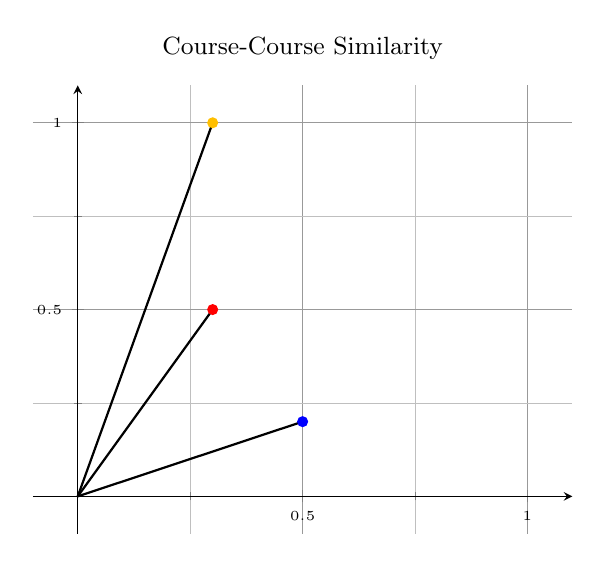
\begin{tikzpicture}
\begin{axis}[
    xmin=0, xmax=1,
    ymin=0, ymax=1,
    xtick={0,0.5,1},
    ytick={0,0.5,1},
    grid=both,
    grid style={line width=0.2pt, draw=gray!50},
    major grid style={line width=0.4pt,draw=gray!80},
    minor tick num=1,
    axis line style={-},
    axis lines=middle,
    enlargelimits=true,
    ticklabel style={font=\tiny},
    label style={font=\small},
    title={Course-Course Similarity},
    title style={font=\small,align=center},
    nodes near coords={
        \pgfmathprintnumber{\pgfplotspointmeta}
    },
    every node near coord/.append style={
        anchor=west,
        font=\footnotesize,
        yshift=2pt, % adjust vertical position of the label
        xshift=-5pt % adjust horizontal position of the label
    }
]
\addplot[
    scatter,
    only marks,
    mark=*,
    mark size=2pt,
    scatter src=explicit,
    scatter/use mapped color={draw opacity=0,fill=mapped color}
]
table[x=x, y=y, meta=meta] {
    x y meta
    0.5 0.2 1
    0.3 1 2
    0.3 0.5 3
};

\draw[thick,-] (axis cs:0.5,0.2) -- (axis cs:0,0);
\draw[thick,-] (axis cs:0.3,1) -- (axis cs:0,0);
\draw[thick,-] (axis cs:0.3,0.5) -- (axis cs:0,0);

\end{axis}
\end{tikzpicture}
\caption{KNN Model}
\end{figure}

\noindent Use the KNN model to calculate the cosine distance between the red course and all other courses. 

\begin{table}[H]
\center
\begin{tabular}{|c|c|}
\hline
\textbf{Course} & \textbf{Cosine Distance} \\
\hline
yellow & 0.25 \\
blue & 0.4 \\
\hline
\end{tabular}
\caption{Predicted Distances}
\end{table}

\noindent After calculating the cosine distances for all courses, select the top most similar courses.

\section{Hybrid Course Recommendation}
\begin{enumerate}
    \item \textsf{Loaded the cleaned dataset.}
    \item \textsf{Combined the results from TF-IDF and KNN approaches using 
    a hybrid recommendation system.}
    \item \textsf{Returned the top N recommended courses for the given user, 
    integrating recommendations from both TF-IDF and KNN approaches.}
\end{enumerate}

\vspace{25pt}
\subsection{The combination of TF-IDF and KNN}

Set the weights and normalize the matrices of TF-IDF and KNN.
\begin{table}[H]
    \centering
    \vspace{10pt}
    \begin{tabular}{|c|c|c|c|c|c|}
        \hline
        & \textbf{User 1} & \textbf{User 2} & \textbf{User 3} & \textbf{User 4} & \textbf{User 5} \\
        \hline
        \textbf{Course 1} & 1.00 & 3.75 & 2.00 & 2.50 & 3.25 \\
        \hline
        \textbf{Course 2} & 2.25 & 2.75 & 1.75 & 1.50 & 1.87 \\
        \hline
        \textbf{Course 3} & 1.00 & 1.40 & 1.95 & 4.55 & 4.45 \\
        \hline
    \end{tabular}
    \caption{Before the normalization}
    \vspace{10pt}
    \begin{tabular}{|c|c|c|c|c|c|}
        \hline
        & \textbf{User 1} & \textbf{User 2} & \textbf{User 3} & \textbf{User 4} & \textbf{User 5} \\
        \hline
        \textbf{Course 1} & 0.167 & 0.626 & 0.334 & 0.417 & 0.543 \\
        \hline
        \textbf{Course 2} & 0.486 & 0.594 & 0.378 & 0.324 & 0.404 \\
        \hline
        \textbf{Course 3} & 0.145 & 0.204 & 0.284 & 0.662 & 0.647 \\
        \hline
    \end{tabular}
    \caption{After the normalization}
\end{table}

\noindent Stack arrays in sequence horizontally

\begin{table}[htbp]
    \centering
    \begin{minipage}[t]{0.4\textwidth} % Adjust the width as needed
        \centering
        \begin{tabular}{|c|c|c|}
        \hline
        & Column 1 & Column 2 \\
        \hline
        Row 1 & 0.1 & 0.2  \\
        Row 2 & 0.3 & 0.4 \\
        Row 3 & 0.5 & 0.6 \\
        \hline
        \end{tabular}
        \caption{Matrix 1}
    \end{minipage}
    \hspace{20pt} % Adjust the horizontal space between tables
    \begin{minipage}[t]{0.4\textwidth} % Adjust the width as needed
        \centering
        \begin{tabular}{|c|c|}
        \hline
        & Column 3\\
        \hline
        Row 1 & 0.7 \\
        Row 2 & 0.8 \\
        Row 3 & 0.9 \\
        \hline
        \end{tabular}
        \caption{Matrix 2}
    \end{minipage}
\end{table}

\begin{table}[htbp]
    \centering
    \begin{tabular}{|c|c|c|c|}
    \hline
    & Column 1 & Column 2 & Column 3 \\
    \hline
    Row 1 & 0.1 & 0.2 & 0.7 \\
    Row 2 & 0.3 & 0.4 & 0.8 \\
    Row 3 & 0.5 & 0.6 & 0.9 \\
    \hline
    \end{tabular}
    \caption{Stacked Matrix}
\end{table}

\subsection{The process of Recommendation}

We apply Nearest Neighbors to the stacked matrix to get the final recommendation.
Nevertheless, the process of recommendation is the same as the KNN approach.

\newpage

\section{Evaluation}

By following this evaluation process, developers and researchers can measure and improve the 
effectiveness of recommendation systems in providing personalized and relevant recommendations to users.

\begin{enumerate}
    \item \textsf{Consider users who have taken more than one course.}
    \item \textsf{The training and testing datasets are splitted by identifying the ratio.}
    \item \textsf{Allow the model to familiarize itself with the training dataset to ensure there is no bias.}
    \item \textsf{Predict the courses for all users using the trained model.}
    \item \textsf{Calculate the accuracy by measuring the similarities between the predicted courses and the actual test courses.}
    \item \textsf{Investigate the results and adjust the parameters to enhance the quality of the system.}
\end{enumerate}

\subsection{Training and Testing}

In designing the training and testing split, several considerations can be made to ensure an effective 
evaluation of the recommendation system. These considerations include:

\begin{enumerate}
    \item \textsf{\textbf{Consider only users who have taken more than 1 course: }
    This step ensures that you have enough data from each user for meaningful analysis.}
    \item \textsf{\textbf{Divide the courses into 2 parts individually according to the specified proportions: }
    This ensures that each user's data is divided according to the specified proportion.}
    \item \textsf{\textbf{Split the dataset corresponding to the curriculum from step 2: }
        This ensures that the dataset is approximately divided into two parts: one for training and one for testing.}
\end{enumerate}

\subsection{Accuracy Measurement}
There are two performance measurements in total including \textit{hit rate} and \textit{f1 score}.

\subsubsection{Hit Rate}
Hit Rate is calculated as follows:

\begin{equation}
    \text{HitRate} = \frac{\texttt{Number of hit users}}{\texttt{All users}}
\end{equation}

\noindent A larger value of recommended courses can potentially improve the hit rate because it provides more opportunities to include relevant items. Therefore, the performance of the hit rate indeed depends on the number of recommended courses.


\subsubsection{F1 Score}

Recall, Precision, and F1 Score can use the following formulas:

\begin{equation}
    Recall = \frac{\texttt{Number of correctly predicted items}}{\texttt{Total number of relevant items}}
\end{equation}

\begin{equation}
    Precision = \frac{\texttt{Number of correctly predicted items}}{\texttt{Total number of recommended items}}
\end{equation}

\begin{equation}
    F1\_score = \frac{2⋅Precision⋅Recall}{Precision+Recall}
\end{equation}

\begin{itemize}
    \item \texttt{Number of correctly predicted items - The course that system predict correctly.}
    \item \texttt{Total number of relevant items - The courses that have been taken by the user from the course recommendation system}
    \item \texttt{Total number of recommended items - All courses that the recommendation system suggests for user}
\end{itemize}

\noindent To find the average F1 score from all users by

\begin{equation}
    \text{$F1\_score_{average}$} = \frac{\sum_{i=1}^{n}F1\_score_{i}}{\texttt{Number of Users}}
\end{equation}

\noindent The harmonic mean nature makes sure if either Precision or Recall has a really high value, then it does not dominate the score. F1 Score has a high value when both precision and recall values are close to 1.
\chapter{\ifproject%
\ifenglish Experimentation and Results\else การทดลองและผลลัพธ์\fi
\else%
\ifenglish System Evaluation\else การประเมินระบบ\fi
\fi}

In this section, we delve into the experimentation phase of our project, where 
the proposed methodologies were put to the test, and their efficacy was evaluated. 
The primary objective was to assess the performance and suitability of the 
recommendation system in providing personalized course recommendations to users.

\section{Data Preparation}

\subsection{Import Datasets}
The dataset provided by the developer is required to be a csv format and consists of two main components:
\begin{minted}[frame=lines, fontsize=\footnotesize]{python}
import pandas as pd
i_data = pd.read_csv('https://startg2545.github.io/item_tutorial.csv')
ui_data = pd.read_csv('https://startg2545.github.io/user_item_tutorial.csv')
\end{minted}

\subsection{Import the Classes}

First of all, import one of these classes from the isne\_recommendation 
module that you desire to evaluate the model.

\begin{minted}[frame=lines, fontsize=\footnotesize]{python}
from isne_recommendation import TfidfLinearKernel, FeatureRatingsKNN, Hybrid
\end{minted}

\subsection{Fit the Model}

The fit function is responsible for adjusting the internal parameters of the model 
to minimize the difference between the predicted outputs and the actual outputs 
(also known as the ground truth) in the training data.

\begin{minted}[frame=lines, fontsize=\footnotesize]{python}
model = TfidfLinearKernel.fit(i_data)
model = FeatureRatingsKNN.fit(ui_data)
model = Hybrid.fit(i_data, ui_data)
\end{minted}

\newpage
\section{Split the Data for training and testing}

The \textit{train-test split} is a common technique used in machine learning to evaluate the 
performance of a model on unseen data. This technique involves splitting the dataset 
into two subsets: one for training the model and another for testing its performance

\begin{minted}[frame=lines, fontsize=\footnotesize]{python}
train, test = TfidfLinearKernel.train_test_split(ui_data)
\end{minted}

\section{Evaluate the model}

Model evaluation is a crucial step in machine learning to assess the performance and 
effectiveness of a trained model on unseen data. The model evaluation function involves 
using various metrics and techniques to measure how well the model generalizes to new data.

\begin{minted}[frame=lines, fontsize=\footnotesize]{python}
# Calculate the hit rate of the model
hit_rate = TfidfLinearKernel.hit_rate(train, test, i_data, model)
hit_rate = FeatureRatingsKNN.hit_rate(train, test, model)
hit_rate = Hybrid.hit_rate(train, test, i_data, model)
# Calculate the F1 score of the model
f1_score = TfidfLinearKernel.f1_score(train, test, i_data, model)
f1_score = FeatureRatingsKNN.f1_score(train, test, model)
f1_score = Hybrid.f1_score(train, test, i_data, model)
\end{minted}

\section{Performance Evaluation}

\begin{enumerate}
    \item \textbf{First Approach}:
    \begin{itemize}
        \item Hit Rate Accuracy: 14.69\%
        \item F1 Score Accuracy: 2.58\%
    \end{itemize}
    \item \textbf{Second Approach}:
    \begin{itemize}
        \item Hit Rate Accuracy: 48.24\%
        \item F1 Score Accuracy: 7.92\%
    \end{itemize}
    \item \textbf{Hybrid Approach}:
    \begin{itemize}
        \item Hit Rate Accuracy: 69.18\%
        \item F1 Score Accuracy: 11.62\%
    \end{itemize}
\end{enumerate}
\ifproject
\chapter{\ifenglish Conclusions and Discussions\else บทสรุปและข้อเสนอแนะ\fi}

\section{\ifenglish Conclusions\else สรุปผล\fi}

นศ. ควรสรุปถึงข้อจำกัดของระบบในด้านต่างๆ ที่ระบบมีในเนื้อหาส่วนนี้ด้วย

\section{\ifenglish Challenges\else ปัญหาที่พบและแนวทางการแก้ไข\fi}

ในการทำโครงงานนี้ พบว่าเกิดปัญหาหลักๆ ดังนี้

\section{\ifenglish%
Suggestions and further improvements
\else%
ข้อเสนอแนะและแนวทางการพัฒนาต่อ
\fi
}

ข้อเสนอแนะเพื่อพัฒนาโครงงานนี้ต่อไป มีดังนี้

\fi

\bibliography{myReport}

\ifproject

\normalspacing
\appendix
\chapter{Technical Implementation Details}

This appendix provides additional technical details and information 
related to the implementation of the \textsf{recommendation system} aimed at 
facilitating course recommendations tailored to individual user 
interests on e-Learning platforms.

\section{Data Collection and Preprocessing}

We collected user interaction data from the e-Learning platform, 
including user ratings, course enrollments, and browsing history. 
The data were preprocessed to remove duplicates, handle missing 
values, and ensure consistency.

\section{Content-Based Filtering}

In the content-based filtering approach, we utilized the TF-IDF 
(Term Frequency-Inverse Document Frequency) technique to extract 
relevant features from course descriptions and user preferences. 
We then applied feature weighting and cosine similarity to 
recommend courses based on similarity to the user's preferences.

\section{Collaborative Filtering}

For collaborative filtering, we employed the K-Nearest Neighbors 
(KNN) algorithm to identify similar users or courses based on their 
interaction patterns. We calculated similarities between users or 
courses and generated recommendations by considering the preferences 
of similar users.

\section{Hybrid Approach}

The hybrid approach combines content-based and collaborative filtering 
techniques to leverage the strengths of both methods. We integrated the 
recommendations generated from both approaches using a weighted or ensemble 
method to provide more personalized and accurate course suggestions.

\section{Model Evaluation}

We evaluated the performance of the recommendation system using standard 
metrics such as accuracy, precision, recall, and F1-score. Additionally, 
we conducted A/B testing or user studies to assess user satisfaction and 
the effectiveness of the recommendations in improving the user experience 
and content discovery on the e-Learning platform.

\chapter{Model Training and Evaluation}

This appendix outlines the key aspects of model training, evaluation metrics, and challenges addressed during the development of the recommendation system.

\section{Model Training}

The recommendation system model was trained using various machine learning algorithms, including content-based filtering, collaborative filtering, and hybrid approaches. Training involved feature extraction, algorithm selection, hyperparameter tuning, and data preparation.

\section{Evaluation Metrics}

Performance evaluation utilized metrics such as accuracy, precision, recall, F1-score, and hit rate to assess the system's effectiveness in recommending relevant courses based on user preferences and interactions.

\section{Challenges and Solutions}

Challenges encountered included data sparsity~\cite{Tian2019}, cold start problem~\cite{Gope2017}, scalability issues, and algorithm complexity. Solutions included data augmentation, cold start handling techniques, scalability improvements, and algorithmic enhancements.

\ifglossary\glossarypage\fi

\ifindex\indexpage\fi

\begin{biosketch}
\begin{figure}[H]
\center
  \begin{minipage}{0.45\textwidth}
    \begin{center}
      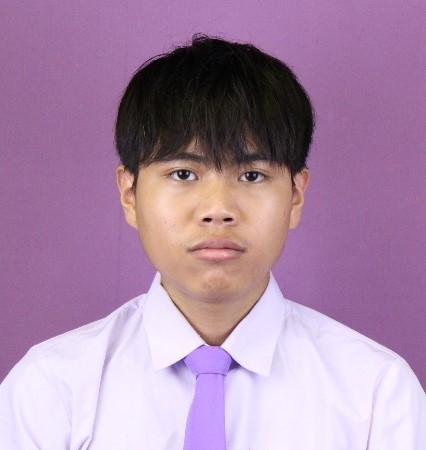
\includegraphics[width=1.5in]{./img/newin_photo.jpg}
    \end{center}
    \begin{center}
      \textsf{Name: Newin Yamaguchi} \\
      \textsf{Affiliation: Chiang Mai University} \\
    \end{center}
  \end{minipage}
  \begin{minipage}{0.45\textwidth}
    \begin{center}
      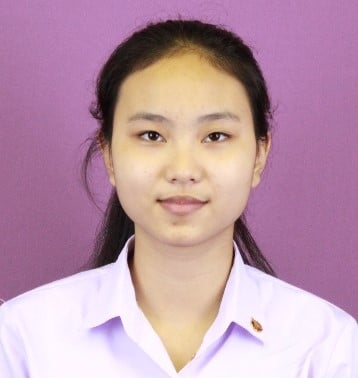
\includegraphics[width=1.5in]{./img/may_photo.jpg}
    \end{center}
    \begin{center}
      \textsf{Name: Patcharaporn Satantaipop} \\
      \textsf{Affiliation: Chiang Mai University} \\
    \end{center}
  \end{minipage}
\end{figure}

\textsf{Newin and Patcharaporn are students at the Department of Computer 
Engineering, Chiang Mai University, specializing in machine learning 
and algorithms. We are currently in the fourth-year of Bachelor's Degree.
With a passion for data science, we have dedicated our career to 
exploring innovative solutions to motivate students to become more
addicted to self-learning.}

\textsf{Our current project focuses on the development of a Recommendation 
System for e-Learning platforms. Recognizing the challenges associated 
with online learning. We aim to investigate diverse models to facilitate 
course recommendations tailored to individual user interests. By leveraging 
a hybrid approach that combines content-based and collaborative filtering 
techniques, we aim to enhance the content discovery process and improve user 
satisfaction in online education.}

\textsf{Overall, Newin and Patcharaporn are dedicated and driven researchers 
committed to making meaningful contributions to the field of Computer 
Engineering. Our recommendation system project for e-Learning 
platforms represents an ongoing commitment to improving online 
education and enhancing the learning experience for students worldwide.}
\end{biosketch}

\fi

\end{document}